\section{Implementation}
	(Note: all code files are available at:
	
	\texttt{https://github.com/ARDivekar/ES\_Project\_Wireless\_Robot/tree/master/es\_project}).
	\\
	
	Once we have connected the Raspberry Pi to the various hardware modules and ensured that the \textit{Raspbain Jesse} installation and \textit{Django server} are working, we may then proceed to create the following code files in a directory \texttt{es\_project} in the home directory of the Raspbian installation. 
	

%	\clearpage
%	\begin{figure}
%		\centering
%		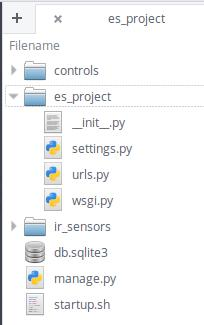
\includegraphics[width=0.3\linewidth]{es_project_directory_1}
%		\caption{}
%		\label{fig:es_project_directory_1}
%	\end{figure}
	
	\begin{figure}
		\hfill
		\subfigure[Main directory \texttt{es\_project/}] {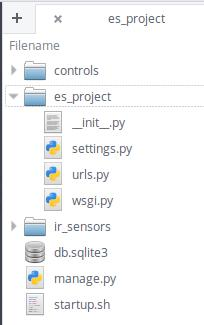
\includegraphics[height=6cm]{es_project_directory_1}}
		\hfill
		\subfigure[Sub directory  \texttt{controls/}]{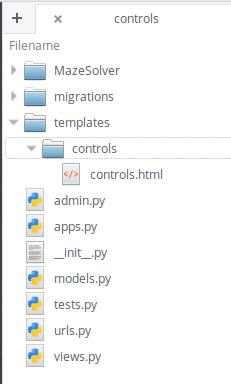
\includegraphics[height=5cm]{es_project_directory_2}}
		\hfill
		\subfigure[Sub directory  \texttt{ir\_sensors/}]{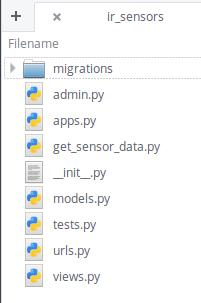
\includegraphics[height=5cm]{es_project_directory_3}}
		\hfill
		\subfigure[Sub directory  \texttt{MazeSolver/}]{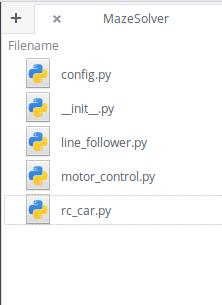
\includegraphics[height=5cm]{es_project_directory_4}}
		\hfill
		\caption{Django project directory layout}
	\end{figure}
	
%	\begin{figure}
%		\centering
%		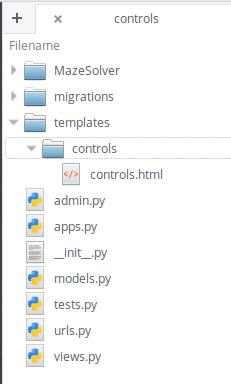
\includegraphics[width=0.3\linewidth]{es_project_directory_2}
%		\caption{}
%		\label{fig:es_project_directory_2}
%	\end{figure}

	
	As a reference, in general the steps outlines in the Django tutorial \cite{DjangoTutorial} should be followed, but some files were modified by us; those changes have been included below.
	
	\begin{description}[font=\quad $\circ$, topsep=6pt, itemsep=3em]
		\item \texttt{es\_project/startup.sh}:
		
			% Source: https://www.sharelatex.com/learn/Code_listing
			\lstinputlisting[language=bash]{"./es_project/startup.sh"}
			
			The initial code in this file is used to retrieve the IP address the Pi3 is connected, to using Linux's \texttt{ifconfig} command. We try both \texttt{wlan0} and \texttt{wlan1} (if we had connected an external USB Wifi dongle), and we use whichever is not empty. 
			
			Once we have retrieved this IP address, we use it to start the Django server by executing \texttt{manage.py runserver}. We pass the IP address discovered as an argument, and use port 2. Thus, when we access the GUI, we would do so from an IP address such as \texttt{192.168.1.100:2/}.
		
		
		
		\item \texttt{es\_project/es\_project/settings.py}:
			% Source: https://www.sharelatex.com/learn/Code_listing
			\lstinputlisting[language=python]{"./es_project/es_project/settings.py"}
			
			We have modified the code here to add the function \texttt{get\_current\_ip\_address\_str()}, which we use to get the IP address of the connection using the \texttt{pyiface} package and the regular expressions package \texttt{re}. We then add this to \texttt{ALLOWED\_HOSTS} in the next line.


		\clearpage
		\item \texttt{es\_project/es\_project/urls.py}		
			% Source: https://www.sharelatex.com/learn/Code_listing
			\lstinputlisting[language=python]{"./es_project/es_project/urls.py"}
			
			In this file we add the various urls which we use to access the various functions. The main one is \texttt{controls}, which we would use to access the GUI as: \texttt{192.168.1.100:2/controls} and the IR sensor feed at \texttt{192.168.1.100:2/ir\_sensors}.
			
			
			
		\item \texttt{es\_project/controls/urls.py}
			\lstinputlisting[language=python]{"./es_project/controls/urls.py"}
		\clearpage
		\item \texttt{es\_project/controls/views.py}
			\lstinputlisting[language=python]{"./es_project/controls/views.py"}
			
			The \texttt{controls/} folder is an "application" in our Django project, which we use to load the GUI and send requests to it from the URL \texttt{192.168.1.100:2/controls}. 
			
			For this we need to accept and route controls such as \texttt{192.168.1.100:2/controls/left}. We use \texttt{controls/urls.py} to route the requests and we use the function \texttt{controls(..., direction)} in \texttt{controls/views.py} to actually call the code from the \texttt{MazeSolver/rc\_car.py} file.
			
		\clearpage
		\item \texttt{es\_project/controls/MazeSolver/config.py}
			\lstinputlisting[language=python]{"./es_project/controls/MazeSolver/config.py"}
		
		\item \texttt{es\_project/controls/MazeSolver/rc\_car.py}
			\lstinputlisting[language=python]{"./es_project/controls/MazeSolver/rc_car.py"}
			
			\texttt{/MazeSolver/config.py} is used to denote which pins are used for the motors and IR sensors in a more human-readable manner. \texttt{/MazeSolver/rc\_car.py} performs all the movement functions that are standard with an RC controller car with two wheels (e.g. to move forward, both wheels must turn in the forward direction, to turn right, the right wheel must move forward and the left wheel must move backwards, etc.). We make \texttt{RPi.GPIO} package to control the motors by setting the Raspberry Pi3's General-Purpose Input/Output pins HIGH or LOW.
		
		
		
		
		\item \texttt{es\_project/ir\_sensors/urls.py}
			\lstinputlisting[language=python]{"./es_project/ir_sensors/urls.py"}
		
		\item \texttt{es\_project/ir\_sensors/views.py}
			\lstinputlisting[language=python]{"./es_project/ir_sensors/views.py"}
		\clearpage		
		\item \texttt{es\_project/ir\_sensors/get\_sensor\_data.py}
			\lstinputlisting[language=python]{"./es_project/ir_sensors/get_sensor_data.py"}
		
			The \texttt{ir\_sensors/} application in Django is located at \texttt{192.168.1.100:2/ir\_sensors} (or the equivalent). It uses the \texttt{RPi.GPIO} package to fetch the data from the IR sensors. We return it as a string of values, e.g. "010" (this would denote that the middle IR sensor is triggered, indicating a white/bright surface below).
		
		
		
	
		\item \texttt{es\_project/controls/templates/controls/controls.html}
			\lstinputlisting[language=HTML]{"./es_project/controls/templates/controls/controls.html"}
		
		This is the page which actually displays the GUI to the user who visits the URL  \texttt{192.168.1.100:2/controls} (or the equivalent). We show the basic buttons, laid out in a grid using CSS3 Bootstrap and HTML. 
		
		The \texttt{<script>} tag defines the function \texttt{getIRvals()}, which when called sends an AJAX request to \texttt{192.168.1.100:2/ir\_sensors} and retrieves the current IR sensor readings ("010", etc). We use \texttt{setInterval(...)} to perform the AJAX call in a loop every 0.5 seconds, thus updating the values retrieved from the IR sensors every 0.5 seconds.
		
		On clicking one of the buttons \textit{"Forward", "Backward", "Left", "Right" or "Stop"}, the corresponding value of \textit{direction} is passed to \texttt{es\_project/controls/views.py}, which in turn calls the corresponding function in \texttt{es\_project/controls/MazeSolver/rc\_car.py}, which sets the corresponding GPIO pins HIGH or LOW, thus causing the motors to move and draw power from the 9v batteries. We can sense the underlaying terrian via the IR sensor readings.
		
		
		\begin{figure}
			\centering
			\includegraphics[width=0.4\linewidth]{"GUI_on_mobile.png"}
			\caption{GUI as seen on an Android device connected to the same Wireless LAN as the rover.}
			\label{fig:GUI_on_mobile}
		\end{figure}			
			
		
		\begin{figure}
			\centering
			\includegraphics[width=0.8\linewidth]{"GUI_on_desktop.jpg"}
			\caption{GUI as seen from a desktop computer connected to the same Wireless LAN as the rover.}
			\label{fig:GUI_on_desktop}
		\end{figure}	
		
	\end{description}
